\documentclass[compress,9pt,xcolor=svgnames]{beamer}
% BEFORE YOU COMPILE IT, READ THE FOLLOWING
% In order to have landscape layout, press "Options" in the menu of WinEdt, then "Execution Modes"-"Console Applications" tab-choose "Default" for "paper size and orientation" for dvi2ps and ps2pdf
% table of contents, overlays and hyperlinks DON'T work with LaTeX+dvi2pdf and pdfLaTeX doesn't work with eps
% Please use latex+dvi2ps+ps2pdf instead. Sometimes you need to run latex twice and then dvi2ps+ps2pdf
% option "compress" in the "documentclass line" compresses the headline, footline and side bars. Default option is "uncompress".

\usepackage{graphics,fancybox,amsmath}
\usepackage{setspace}
\usepackage[ruled,vlined,commentsnumbered]{algorithm2e}
\usepackage{multirow}
\usepackage{setspace}
% \usepackage{underbrace}
\usepackage{mathtools}

\thinmuskip=10mu
%\usepackage{times}
% font packages: sans avant bookman chancery charter helvet newcent palatino utopia
\newcommand{\thedate}{November 15, 2016}
\newcommand{\norm}[1]{\left\|\,#1\,\right\|}
\newcommand{\Rset}{{\rm I}\!{\rm R}}
\newcommand{\dis}{\displaystyle}
\newcommand{\tr}{\mathrm{T}}
\newcommand{\bx}{\mathbf{x}}
\newcommand{\bff}{\mathbf{f}}
\newcommand{\bG}{\mathbf{G}}
\newcommand{\bg}{\mathbf{g}}
\newcommand{\bu}{\mathbf{u}}
\newcommand{\by}{\mathbf{y}}
\newcommand{\bxh}{\widehat{\mathbf{x}}}
\newcommand{\byh}{\hat{\mathbf{y}}}
\newcommand{\bffh}{\hat{\mathbf{f}}}
\newcommand{\bGh}{\hat{\mathbf{G}}}
\newcommand{\bgh}{\hat{\mathbf{g}}}
\newcommand{\bxb}{\bar{\mathbf{x}}}
\newcommand{\diag}{\mathrm{diag}}
\newcommand{\xh}{\hat{x}}
\newcommand{\bz}{\mathbf{0}}
\newcommand{\bK}{\mathbf{K}}
\newcommand{\bk}{\mathbf{k}}
\newcommand{\Deltah}{\hat{\Delta}}
\newcommand{\be}{\mathbf{e}}
\newcommand{\bB}{\mathbf{B}}
\newcommand{\bBh}{\mathbf{\widehat{B}}}
\newcommand{\bA}{\mathbf{A}}
\newcommand{\bAh}{\mathbf{\widehat{A}}}


\graphicspath{{./fig/}}

\mode<presentation>{
    \usetheme{Frankfurt}
%    \useoutertheme{umbcfootline}}
    % themes: Antibes Bergen Berkeley Berlin Boadilla Copenhagen Darmstadt Dresden Frankfurt Goettingen Hannover Ilmenau Juanlespins Luebeck Madrid Malmoe Marburg Montpellier Paloalto Pittsburgh Rochester Singapore Szeged Warsaw
    \definecolor{CalBlue}{RGB}{0,23,203} % define a new color using the RGB code
    \definecolor{BlockTitleGreen}{RGB}{108,178,108}
    \definecolor{BlockBodyWhite}{RGB}{238,238,238}
    %\definecolor{BlockBodyWhite}{RGB}{240,248,240}
    \definecolor{BlockBodyBlue}{RGB}{230,235,240}
    %\definecolor{DavisBlue}{RGB}{0,73,132}
    \definecolor{DaMarron}{RGB}{125,0,0}
    \definecolor{DaDarkGray}{RGB}{81,81,81}
    \definecolor{DaRed2}{RGB}{96,25,134}
    \definecolor{DavisGold}{RGB}{189,146,0}
    \definecolor{LightPink}{RGB}{235,104,119}
    \definecolor{BoxBlue}{RGB}{0,28,88}
    \definecolor{LightYellow}{RGB}{255,247,153}
    \definecolor{DarkBlue}{RGB}{8,107,175}
    \definecolor{DarkRed}{RGB}{236,104,67}

    % gradient background from 10% blue to white
    \usecolortheme[named=DaMarron]{structure} % assigns the color used for the structural elements
    %\useinnertheme{rectangles} % other options: default, circles, rounded
    %\useoutertheme[subsection=false]{miniframes} % puts a mini bar showing the sections of the presentation on top of each frame
    %\usecolortheme{dolphin} % without this command, the mini bar won't have the same color as the specified color for structural elements
    %\setbeamertemplate{blocks}[rounded][shadow=true] % changes the shape of the blocks and draw shadows
    \beamertemplatetransparentcovereddynamicmedium % or \beamertemplatetransparentcoveredhigh or \setbeamercovered{transparent}, these commands makes the covered items transparent (opacities are different)
    \setbeamertemplate{navigation symbols}{} % inserts only the "go to", "back" and "forward" symbols
    %\setbeamertemplate{footline}[frame number] % insert page number in footline
    \usefonttheme[onlymath]{serif} % use serif for equations and math symbols only
    \usefonttheme[onlysmall]{structureitalicserif} % changes the font for small texts such as the section names in the mini bar
    %\setbeamercolor{block title}{fg=blue} % set the color of the block title to be blue instead of the structure color
    \setbeamerfont{title}{size*={11}{15},series=\bfseries} % set the font size of the title to 11 pt bold with 15 as the baselineskip
    \setbeamerfont{author}{size=\large}
    \setbeamerfont{institute}{size=\large}
    \setbeamerfont{date}{size=\large}
    \setbeamerfont{frametitle}{size=\normalsize,series=\bfseries}
    \setbeamerfont{block title}{size=\normalsize,series=\bfseries}
    %\setbeamercolor{title}{fg=Purple}
    \setbeamercolor{author}{fg=black} % set the color of the author to the same as structural elements
    \setbeamercolor{institute}{fg=DaMarron}
    \setbeamercolor{date}{fg=black}
    \setbeamercolor{section in toc}{fg=structure}
    \setbeamercolor{subsection in toc}{fg=structure}
    \setbeamercolor{block}{fg=white}
    %\setbeamercolor{frametitle}{fg=Purple}
    \setbeamercolor{navigation symbols dimmed}{fg=LightPink}
    \setbeamercolor{navigation symbols}{fg=LightPink}
    \setbeamercolor{navigation symbols dimmed}{bg=LightPink}
    \setbeamercolor{navigation symbols}{bg=LightPink}

    \setbeamertemplate{itemize item}[circle]% triangle ball square circle
    \setbeamerfont{itemize item}{size=\normalsize}
    \setbeamercolor{itemize item}{fg=DaMarron}
    \setbeamerfont{itemize/enumerate body}{size=\normalsize}
    \setbeamercolor{itemize/enumerate body}{fg=Black}
    \setbeamertemplate{itemize subitem}[triangle]
    \setbeamerfont{itemize subitem}{size=\normalsize}
    \setbeamercolor{itemize subitem}{fg=DaDarkGray}
    \setbeamerfont{itemize/enumerate subbody}{size=\normalsize}
    \setbeamercolor{itemize/enumerate subbody}{fg=Black}
    \setbeamertemplate{itemize subsubitem}[triangle]
    %\setbeamertemplate{itemize subsubitem}[circ]
    \setbeamerfont{itemize subsubitem}{size=\tiny}
    \setbeamercolor{itemize subsubitem}{fg=gray}
    \setbeamerfont{itemize/enumerate subsubbody}{size=\normalsize}
    \setbeamercolor{itemize/enumerate subsubbody}{fg=Black}
    \setbeamercolor{postit}{bg=LightYellow, fg=black}
    %\setbeamercolor{postit}{bg=Moccasin, fg=black}
    %\setbeamercolor{bgcgreen}{bg=BlockTitleGreen, fg=white}
    %\setbeamercolor{bgcwhite}{bg=BlockBodyWhite,fg=DarkSlateBlue}
    \setbeamercolor{White}{bg=White,fg=White}

    \setbeamersize{text margin left=8mm}
    \setbeamersize{text margin right=8mm}

      \leftmargini 1.5em % indent for item
      \leftmarginii 1.5em % indent for subitem
      \leftmarginiii 1.5em % indent for subsubitem


%This sets the bottom "footline" of every slide to be something fancy
%-----------------------------------------------------------------------------
  \setbeamertemplate{footline}{
  \leavevmode

  \hbox{\begin{beamercolorbox}[wd=.25\paperwidth,ht=2.5ex,dp=1.125ex,leftskip=.3cm,rightskip=.3cm plus1fill]{title in head/foot}%
    \usebeamerfont{author in head/foot}\insertshortauthor
  \end{beamercolorbox}

  \hskip-1mm

  \begin{beamercolorbox}[wd=.25\paperwidth,ht=2.5ex,dp=1.125ex,leftskip=.3cm,rightskip=.3cm plus1fill]{title in head/foot}%
    \usebeamerfont{author in head/foot}\insertshortinstitute
  \end{beamercolorbox}

  \hskip-1mm

  \begin{beamercolorbox}[wd=.256\paperwidth,ht=2.5ex,dp=1.125ex,leftskip=.3cm plus1fill,rightskip=.3cm]{title in head/foot}%
    {\thedate}
  \end{beamercolorbox}

  \hskip-1mm

  \begin{beamercolorbox}[wd=.25\paperwidth,ht=2.5ex,dp=1.125ex,leftskip=.3cm plus1fill,rightskip=.3cm]{title in head/foot}%
    \insertframenumber/\inserttotalframenumber
  \end{beamercolorbox}}

  \vskip0pt

  }
%----------------------------------------------------------------------------

% these will be used later in the title page
\title[Da_16ACC]{Optimization-Based Networked Predictive Control of Process Systems with Control and Communication Constraints}
%SUPERVISORY LOGIC FOR CONTROL OF NETWORKED PROCESS SYSTEMS WITH EVENT-BASED COMMUNICATION}% \vskip creates vertical space, sometimes \vspace is not working
\author[El-Farra $\&$ Xue]{ \vskip -1mm Da Xue and Nael H. El-Farra \vskip0mm}% \structure forces the texts to have the same color as structural elements which is dark blue here
\pgfdeclareimage[height=1.6cm]{logo}{UCD_Seal_YB} % declare "logo" as the name for UCD_Seal_YB
\institute[CHE,\ UC Davis]{ Department of Chemical Engineering\\
            University of California, Davis}
\date[ACC 2016]{ % \vskip-2mm\pgfuseimage{logo}\\ % use the declared image
        \vskip 2mm
    \begin{columns}[c]
    \column{0.04\textwidth}
    \column{0.15\textwidth}
    % \color{BoxBlue}{\setlength{\fboxrule}{0.7pt}\doublebox{\pgfuseimage{logo}}}
    \column{0.60\textwidth}
    \begin{center}
    2016 AIChE Annual Meeting\\
        San Francisco, CA\\
        November 15, 2016
    \end{center}
    \column{0.15\textwidth}
    % \color{BoxBlue}{\setlength{\fboxrule}{0.7pt}\doublebox{\pgfuseimage{logo}}}
    \column{0.06\textwidth}
    \end{columns}
    }

\begin{document}

% this prints title, author etc. info from above
%% FRAME 1
{\beamertemplateshadingbackground{DavisGold!20}{DavisGold!25} % to keep the change of the template local, add { and } right before and after this frame and put the command here
\frame[t]{ % [t] option places the content of the frame on top of the page
    \vskip 4mm
    \titlepage
}}

\section{Introduction}
\subsection*{Feedback control paradigms}
%% FRAME 3
\frame[t]{
  \frametitle{FEEDBACK CONTROL PARADIGMS}
  \vspace{-3mm}
  \begin{block}{Traditional: output transmitted directly and flawlessly to the controller}
    \begin{center}
      \hspace{-0.3in}
      \includegraphics[scale=0.17]<1>{feedback_control}
      \includegraphics[scale=0.12]<2->{feedback_control}
    \end{center}
  \end{block}
    \vskip -1mm
  \begin{block}{Emerging: increasing complexity of the process/controller interface}<only@2->
    \begin{center}
      \includegraphics[scale=0.15]<2->{wireless_sensor_network}
    \end{center}
  \end{block}
}

\subsection*{Feedback control paradigms}
%% FRAME 4
\frame[t]{
  \frametitle{FEEDBACK CONTROL PARADIGMS}
  \vskip -3mm
  \begin{block}{Emerging: increasing complexity of the process/controller interface}
    \begin{center}
      \includegraphics[scale=0.1175]<1>{wireless_sensor_network}
    \end{center}
  \end{block}
  \vskip -1mm
    \begin{block}{Motivation}
        \begin{itemize}
            \item \textcolor[rgb]{0.64,0.00,0.00}{Smart plant} operations\vspace{-0.5mm}
            \begin{itemize}
              \item Advances in actuator and sensor manufacturing technologies\vspace{-0.5mm}
            \end{itemize}
            \item Economic and operational benefits\vspace{-0.5mm}
            \begin{itemize}
              \item Reduced installation and maintenance time and costs\vspace{-0.5mm}
              \item Flexibility and ease of diagnosis and reconfiguration
            \end{itemize}
        \end{itemize}
    \end{block}
  \vskip -1mm
  \begin{block}{Main conflict}
            \vskip -2mm
        \begin{columns}
            \column{0.00\textwidth}
            \column{0.4\textwidth}
            \begin{itemize}
                \item Energy / resource utilization\vspace{-0.5mm}
                \item \textcolor[rgb]{0.64,0.00,0.00}{Minimal} communication
            \end{itemize}
            \column{0.10\textwidth}
            \begin{center}
                \includegraphics[scale=0.1]{vs}
                \end{center}
            \column{0.450\textwidth}
            \begin{itemize}
                \item Stability / performance\vspace{-0.5mm}
                \item \textcolor[rgb]{0.64,0.00,0.00}{Frequent} communication
            \end{itemize}
        \end{columns}
  \end{block}
}


\section{Previous Work}
\subsection*{Quasi Decentralized}
\frame[c]{
  \frametitle{MODEL-BASED NETWORKED CONTROL}
  \vskip -3mm
  \begin{block}{Sun \& El-Farra \scriptsize{(Comput. Chem. Eng., 2008; Ind. Eng. Chem. Res., 2010; Chem. Eng. Sci., 2012)}}
        \begin{columns}[c]
            \column{0.05\textwidth}
            \column{0.4\textwidth}
                \centerline{\includegraphics[scale=0.2]{quasi_decentralized}}

            \column{0.6\textwidth}
                \begin{itemize}
                \item Key architectural features:
                \begin{itemize}
                    \item \textcolor[rgb]{0.64,0.00,0.00}{Model} of the plant embedded
                    \item Model state is \textcolor[rgb]{0.64,0.00,0.00}{updated} when communication is reestablished
                    \item \textcolor[rgb]{0.64,0.00,0.00}{Constant rate} model update 
                \end{itemize}
            \end{itemize}
        \end{columns}  
  \end{block}
  \vskip -1mm
  \begin{block}{Closed-loop properties}
    \vspace{0.5mm}
    \begin{itemize}
        \item Overall stability is guaranteed with reduced communication
        \item Maximum allowable model update period can be explicitly characterized
    \end{itemize}
    \vspace{0.5mm}
  \end{block}
  \vskip -1mm
  \begin{block}{Open issues}    
    \vspace{0.5mm}
    \begin{itemize}
        \item Not robust to disturbances
        \item Controller performance optimization 
        \item Communication cost not accounted for in controller design
    \end{itemize}
    \vspace{0.5mm}
  \end{block}
}

\section{Present work}
\subsection*{Outline of present work}
\frame[c]{
    \frametitle{OUTLINE OF PRESENT WORK}
    \vskip -2mm
    \begin{block}{Scope: Continuous-time process systems}
        \vskip -2mm
        \begin{columns}
            \column{0.00\textwidth}
            \column{0.4\textwidth}
            \begin{itemize}
                \item Plant-model mismatch
            \end{itemize}
            \column{0.60\textwidth}
            \begin{itemize}
                \item Communication resource constraints
            \end{itemize}
        \end{columns}
        \vspace{1mm}
    \end{block}
    \vspace{-2mm}
    \begin{block}{Objectives}
        \begin{itemize}
            \item Development of an optimization-based predictive control framework\vspace{1mm}
            \begin{itemize}
                \item Enforce closed-loop stability%\vspace{1mm}
                \item Simultaneously optimize control and communication performances%\vspace{1mm}
            \end{itemize}
            \item Application to a representative chemical process example
        \end{itemize}
        \vspace{0.5mm}
    \end{block}
    \vspace{-2mm}
    \begin{block}{Approach}
        \begin{itemize}
            \item Design of an auxiliary model-based controller %\vspace{1mm}
            \begin{itemize}
                \item Characterization of the maximum allowable model update period in terms of controller design parameters\vspace{1mm}
            \end{itemize}
            \item Formulation of an optimization-based predictive controller%\vspace{1mm}
            \begin{itemize}
                \item Incorporate communication cost into the cost function%\vspace{1mm} 
                \item Receding horizon implementation
            \end{itemize}
        \end{itemize}
        \vspace{0.5mm}
    \end{block}
}


\subsection*{System description}
\frame[c]{
    \frametitle{NETWORKED PROCESS SYSTEM DESCRIPTION}
    \vskip -3mm
    \begin{block}{Class of systems:}
    \centerline{\begin{beamercolorbox}[wd=2in,center,rounded=true]{postit} $\begin{array}{c}
            \dot{\bx}(t) = \bA\bx(t) + \bB\bu(t)
        \end{array}$
    \end{beamercolorbox}}
    % \vspace{-1mm}

    \begin{itemize}
      \item $\bx\in\mathbb{R}^{n_{\bx}}$: vector of process state variables
      \item $\bu\in\mathbb{R}^{n_{\bu}}$: vector of manipulated inputs
      \item $\bA$, $\bB$: constant state and input matrices
    \end{itemize}
    \vspace{0.5mm}
    \end{block}
    % \vskip -0.5mm
    \begin{block}{Approximate dynamic model:}
    \centerline{\begin{beamercolorbox}[wd=2in,center,rounded=true]{postit} $\begin{array}{c}
            \dot{\bxh}(t) = \bAh\bxh(t) + \bBh\bu(t)
        \end{array}$
    \end{beamercolorbox}}
    % \vskip -0.5mm
    \begin{itemize}
      \item $\bxh\in\mathbb{R}^{n_{\bx}}$: vector of model state variables
      \item $\bAh = \bA - \delta_{\bA}$: approximate model of $\bA$ with uncertainty
      \item $\bBh = \bB - \delta_{\bB}$: approximate model of $\bB$ with uncertainty
    \end{itemize}
    \vspace{0.5mm}
    \end{block}
}


\subsection*{Model-based controller design}
\frame[c]{
    \frametitle{STEP 1: MODEL-BASED NETWORKED CONTROL}
    \vskip -2mm
    \begin{block}{Design of model-based controller using periodic communication}
        \centerline{\begin{beamercolorbox}[wd=3in,center,rounded=true]{postit} $\begin{array}{rcl}
            \dot{\bxh}(t) &=& \bAh\bxh(t) + \bBh\bu(t)\\
            \bu(t) &=& \bK\bxh(t),\ t\in[t_k, t_k+h)\\
            \bxh(t_k) &=& \bx(t_k)
            \end{array}$
        \end{beamercolorbox}}
        \vspace{-1mm}
        \begin{itemize}
            \item $h$: model update period
            \item Asymptotic stabilization of the origin of the closed-loop plant
        \end{itemize}
    \vspace{0.5mm}
    \end{block}
    \vspace{-1mm}

    \begin{block}{Closed-loop system formulation}
        \begin{itemize}
            \item Model estimation error: $\be(t) = \bx(t) - \bxh(t)$\vspace{1mm}
            \item Augmented state: $\xi(t) = [\bx^T(t)\ \be^T(t)]^T$\vspace{2mm}
        \centerline{$\begin{array}{rcl}
            \dot{\xi}(t) &=& \Lambda\xi(t)\\[2mm]
            \xi(t) &=& e^{\Lambda(t - t_k)}(I_se^{\Lambda h}I_s)^k\xi_0 = e^{\Lambda(t - t_k)}M^k\xi_0,\ t\in [t_k, t_{k+1})\\[2mm]
        \end{array}$
        }\vspace{1mm}
            \begin{itemize}
                \item $\xi_0 = \xi(t_0)$, $I_s = \left[\begin{array}{cc}
                        I_{m\times m}   &  O_{m\times m}\\
                        O_{m\times m}   &  O_{m\times m}
                    \end{array}\right]$
            \end{itemize}
        \end{itemize}
        \vspace{0.5mm}
    \end{block}
}

\subsection*{Model-based controller design}
\frame[c]{
    \frametitle{STEP 1: MODEL-BASED NETWORKED CONTROL}
    \vskip -3mm
    \begin{block}{Closed-loop system formulation}
        \begin{itemize}
            \item Model estimation error: $\be(t) = \bx(t) - \bxh(t)$\vspace{1mm}
            \item Augmented state: $\xi(t) = [\bx^T(t)\ \be^T(t)]^T$\vspace{2mm}
        \centerline{$\begin{array}{rcl}
            \dot{\xi}(t) &=& \Lambda\xi(t)\\[2mm]
            \xi(t) &=& e^{\Lambda(t - t_k)}(I_se^{\Lambda h}I_s)^k\xi_0 = e^{\Lambda(t - t_k)}M^k\xi_0,\ t\in [t_k, t_{k+1})\\[2mm]
        \end{array}$
        }\vspace{1mm}
            \begin{itemize}
                \item $\xi_0 = \xi(t_0)$, $I_s = \left[\begin{array}{cc}
                        I_{m\times m}   &  O_{m\times m}\\
                        O_{m\times m}   &  O_{m\times m}
                    \end{array}\right]$
            \end{itemize}
        \end{itemize}
        \vspace{0.5mm}
    \end{block}

    \begin{block}{Stability condition {\scriptsize (Garcia \& Antsaklis, 2003, Sun \& El-Farra, 2008)}}
    \begin{itemize}
        \item Eigenvalues of $M(h)$ are strictly inside the unit circle
        \leftline{\begin{beamercolorbox}[wd=3.8in,center,rounded=true]{postit} $
            M(h) = \left[\begin{array}{cc}
                    I_{m\times m}   &  O_{m\times m}\\
                    O_{m\times m}   &  O_{m\times m}
                \end{array}\right]e^{h\Lambda}\left[\begin{array}{cc}
                    I_{m\times m}   &  O_{m\times m}\\
                    O_{m\times m}   &  O_{m\times m}
                \end{array}\right]$
        \end{beamercolorbox}}
        \item $\lambda_{\max}\{M(\textcolor[rgb]{0.64,0.00,0.00}{K},\textcolor[rgb]{0.64,0.00,0.00}{h},\bA, \bB, \bAh, \bBh)\} < 1$
    \end{itemize}
    \vspace{0.5mm}
    \end{block}
}


\subsection*{step 2}
\frame[t]{
    \frametitle{STEP 2: OPTIMIZATION-BASED CONTROLLER DESIGN}
    \vskip -3mm
    \begin{block}{Finite-horizon optimization problem formulation}
        \centerline{\begin{beamercolorbox}[wd=4in,center,rounded=true]{postit}$\begin{array}{c}
                \displaystyle{\min_{K_k, h_k} J = \int_{t_k}^{t_k+H} [\bxh^T(t)W_{\bxh}\bxh(t) + \bu^T(t)W_{\bu}\bu(t)]dt + \textcolor[rgb]{0.64,0.00,0.00}{\underbrace{\frac{W_h}{h_k}}}}\\
                \hspace{75mm}{\textcolor[rgb]{0.64,0.00,0.00}{\text{\small communication cost}}}
                            \end{array}$
                      \end{beamercolorbox}}
        \hspace{1mm} Subject to:
        \centerline{\begin{beamercolorbox}[wd=3in,center,rounded=true]{postit}$\begin{array}{rl}
                \text{Model dynamics: }&\dot{\bxh}(t) = \bAh\bxh(t) + \bBh\bu(t)\\[2mm]
                \text{Control action: }&\bu(t) = K_k\bxh(t)\\[2mm]
                \text{Stability constraint: }&\lambda_{\max}\{M(K_k, h_k)\} < 1
                            \end{array}$
                      \end{beamercolorbox}}
        % \vspace{0.1mm}
    \end{block}
          \begin{itemize}
            \item $K_k$: controller gain 
            \item $h_k$: model update period
            \item $H$: optimization horizon
            \item $W_{\bxh}$: penalty coefficient on the model state
            \item $W_{\bu}$: penalty coefficient on the control action
            \item $W_h$: penalty coefficient on communication frequency
        \end{itemize} 
}

\subsection*{step 3}
\frame[c]{
    \frametitle{RECEDING-HORIZON IMPLEMENTATION STRATEGY}

    \centerline{\includegraphics[scale=0.6]{flowchart}}
}


\frame[c]{
    \frametitle{RECEDING-HORIZON IMPLEMENTATION}
    \vspace{-2mm}
    \begin{block}{Key features}
    \vspace{0.5mm}
        \begin{itemize}
            \item Choice of penalty coefficients \vspace{1mm}
            \begin{itemize}
              \item Balancing control performance and communication cost\vspace{3mm}
            \end{itemize}
            \item Characterization of feasible region can be done off-line\vspace{1mm}
            \begin{itemize}
                \item $\lambda_{\max}\{M(K, h)\}$\vspace{1mm}
                \item Reduced computation time\vspace{3mm}
            \end{itemize}
            \item Time-varying model update period $h_k$\vspace{1mm}
            \begin{itemize}
              \item Adaptive to changes in operating conditions\vspace{3mm}
            \end{itemize}
            \item Explicitly incorporates communication cost $\frac{W_h}{h_k}$\vspace{1mm}
            \begin{itemize}
                \item Other forms of communication cost can be included
            \end{itemize}
        \end{itemize}
        \vspace{0.2mm}
    \end{block}

}


\section{Simulations}
\subsection{Setup}
\frame[t]{
    \frametitle{ILLUSTRATIVE EXAMPLE}
    \vspace{-0mm}
  \centerline{\includegraphics[scale=0.15]{CSTR}}
  \vspace{2mm}

  \begin{block}{Problem formulation}
  \begin{itemize}
    % \item Reactions: $A\stackrel{k}\longrightarrow B$
    \item Control objectives:%\vspace{1mm}
    \begin{itemize}
      \item Stabilization near open-loop unstable steady state%\vspace{1mm}
      \item Minimal information exchange%\vspace{1mm}
    \end{itemize}
    \item State measurements available%\vspace{1mm}
    \item Manipulated input: $Q$
  \end{itemize}
  \end{block}

}

\frame[t]{
    \frametitle{ILLUSTRATIVE EXAMPLE}
    \vspace{-0mm}
  \centerline{\includegraphics[scale=0.15]{CSTR}}
  \vspace{2mm}
  \begin{block}{Process dynamic model}
                {\small\begin{align*}
                    &\dot{T}=\frac{F}{V}(T_0-T_1) + \frac{-\Delta H}{\rho c_p}k_0e^{\frac{-E}{RT}}C_A + \frac{Q}{\rho c_pV}\\[2mm]
                    &\dot{C}_A=\frac{F}{V}(C_{A0}-C_A) -k_0e^{\frac{-E}{RT}}C_A
            \end{align*}}
            \end{block}
}


\subsection{CSTR}
\frame[t]{
    \frametitle{ILLUSTRATIVE EXAMPLE}
    \vskip -3mm

    \begin{itemize}
        \item Characterization of $\lambda_{\max}\{M(k_1,h)\}$, $k_2 = 2000$, $K = [k_1\ k_2]$
    \end{itemize}

    \centerline{\includegraphics[scale=0.35]{Contour_lambda1}}  

}

\frame[t]{
    \frametitle{ILLUSTRATIVE EXAMPLE}
    \vskip -3mm

    \begin{itemize}
        \item Characterization of $\lambda_{\max}\{M(k_1,h)\}$, $k_2 = 2000$, $K = [k_1\ k_2]$
    \end{itemize}

    \centerline{\includegraphics[scale=0.35]{Contour_lambda2}}  

}

\frame[t]{
    \frametitle{ILLUSTRATIVE EXAMPLE}
    \vskip -3mm

    \begin{itemize}
        \item Characterization of $\lambda_{\max}\{M(k_1,h)\}$, $k_2 = 2000$, $K = [k_1\ k_2]$
    \end{itemize}

    \centerline{\includegraphics[scale=0.35]{Contour_lambda3}}  

}

\frame[t]{
    \frametitle{ILLUSTRATIVE EXAMPLE}
    \vskip -3mm
    \begin{columns}[c]
        \column{0.55\textwidth}
          \begin{itemize}
              \item Characterization of $\lambda_{\max}\{M(K,\hspace{-4pt}h)\}$\vspace{2mm}
              \item Allowable update period $(h_{\min},\hspace{-4pt}h_{\max})$
          \end{itemize}
        \column{0.45\textwidth}
          \leftline{\includegraphics[scale=0.3]{0911_HmaxHmin}}  
    \end{columns}
    \vspace{-2mm}
    \centerline{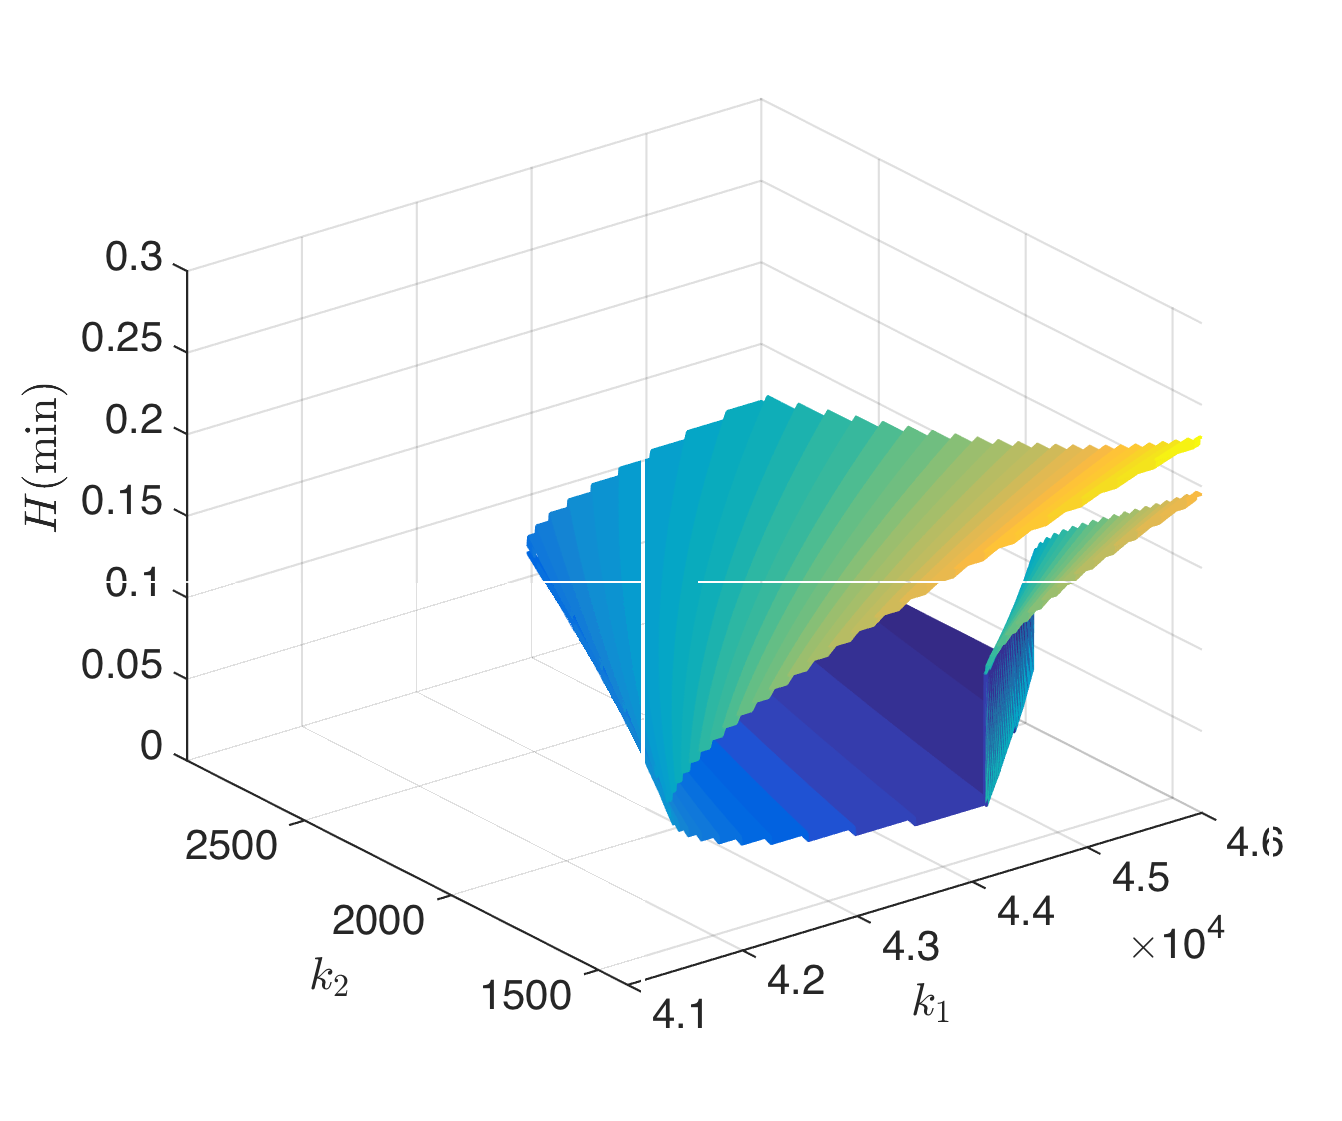
\includegraphics[scale=0.6]{HmaxHmin}}  
}

\subsection*{Performance comparison}
\frame[c]{
    \frametitle{ILLUSTRATIVE EXAMPLE}
    \vskip -3mm
    \begin{block}{Comparison of predictive controllers}
    \vspace{-1mm}
      \begin{columns}[t]
        \column{0.38\textwidth}
          \begin{itemize}
            \item \textcolor{DarkBlue}{With communication cost}
            \begin{itemize}
              \item $W_{\bxh} = W_{\bu} = W_h = 1$\vspace{0.5mm}
              \item $H = 6$min
            \end{itemize}
          \end{itemize}
        
        \column{0.5\textwidth}
          \begin{itemize}
            \item \textcolor{DarkRed}{Without communication cost}
            \begin{itemize}
              \item $J = \int_0^\infty (\bxh^TW_{\bxh}\bxh + \bu^TW_\bu\bu)dt$\vspace{0.5mm}
              \item $W_{\bxh} = W_{\bu} = 1$\vspace{0.5mm}
              \item $h_{\min} = 0.05$min, $h_{\max} = 0.15$min
            \end{itemize}
          \end{itemize}
      \end{columns}
      \vspace{1mm}
    \end{block}
    \vspace{2mm}
    \centerline{\includegraphics[scale=0.22]{CSTR_state}}  
}

\subsection*{Performance comparison}
\frame[c]{
    \frametitle{ILLUSTRATIVE EXAMPLE}
    \vskip -3mm
    \begin{block}{Comparison of predictive controllers}
    \vspace{-1mm}
      \begin{columns}[t]
        \column{0.38\textwidth}
          \begin{itemize}
            \item \textcolor{DarkBlue}{With communication cost}
            \begin{itemize}
              \item $W_{\bxh} = W_{\bu} = W_h = 1$\vspace{0.5mm}
              \item $H = 6$min
            \end{itemize}
          \end{itemize}
        
        \column{0.5\textwidth}
          \begin{itemize}
            \item \textcolor{DarkRed}{Without communication cost}
            \begin{itemize}
              \item $J = \int_0^\infty (\bxh^TW_{\bxh}\bxh + \bu^TW_\bu\bu)dt$\vspace{0.5mm}
              \item $W_{\bxh} = W_{\bu} = 1$\vspace{0.5mm}
              \item $h_{\min} = 0.05$min, $h_{\max} = 0.15$min
            \end{itemize}
          \end{itemize}
      \end{columns}
      \vspace{1mm}
    \end{block}
    \vspace{2mm}
    \centerline{\includegraphics[scale=0.22]{CSTR_U}}  
}


\section{Summary}
\subsection{Summary}
\frame[c]{
    \frametitle{SUMMARY}
    % \vskip 1.5mm
    \begin{itemize}
        \item Continuous-time process systems: \vspace{1mm}

        \begin{itemize}
        \item Communication resource constraints\vspace{1mm}
        \item Plant-model mismatch\vspace{1mm}
        \end{itemize}

        \item Optimization-based predictive control framework:\vspace{1mm}

        \begin{itemize}

            \item Auxiliary model-based controller synthesis\vspace{1mm}
            \begin{itemize}
                \item Characterization of the maximum allowable model update period in terms of controller design parameters\vspace{1mm}
            \end{itemize}

            \item Optimization-based controller design\vspace{1mm}
            \begin{itemize}
                \item Incorporate communication cost into the cost function\vspace{1mm}
                \item Receding horizon implementation\vspace{1mm}
            \end{itemize}

        \end{itemize}
        
        \item Application to a chemical process example

    \end{itemize}

    \begin{block}
        {\begin{center}
            ACKNOWLEDGEMENTS
        \end{center}}
        \vskip -2mm
        \begin{columns}
        \column{0.01\textwidth}
        \column{0.49\textwidth}
    	\begin{itemize}
            \item NSF, CBET-1438456
        \end{itemize}
        \column{0.02\textwidth}
        \column{0.48\textwidth}
        \begin{itemize}
            \item UCD CHMS/CSC Fellowship
        \end{itemize}
	\end{columns}
    \end{block}
}

\end{document}}

